%        File: prac2.tex
%     Created: Sun Mar 03 05:00  2019 S
% Last Change: Sun Mar 03 05:00  2019 S
%
\documentclass[a4paper, 12pt]{article}
\usepackage[]{amsmath}
\usepackage{amssymb}
\usepackage{float}
\usepackage[]{graphicx}
\usepackage{subfig}
\usepackage{caption}


\title{Control Systems 4A Practical 2 Report}
\author{Ruan de Bruyn, 216054484 \and Quintin Kruger, 216008466}

\begin{document}

\pagenumbering{gobble}
\begin{titlepage}
  \maketitle
\end{titlepage}

\pagenumbering{roman}
\tableofcontents
\newpage
\pagenumbering{arabic}

\section{Question 1}
\subsection{Input-Output form}
From the schematic representation of a DC motor, we can use KVL in order to
find the input-output relationships of all the components in the circuit
expressed as voltages. This leaves us with

\begin{equation}
  \begin{array}{rcl}
    v & = & V_R + V_L + e \\
    & = & Ri + L\dot i + K \dot\theta
  \end{array}
  \label{eq:KVL}
\end{equation}

\noindent Note that \eqref{eq:KVL} is a better representation for us to solve
the input-output equations; the current through the DC Motor is also the
same current through the other components. From theory, we can relate the
back-emf of the motor to its rotational speed $\dot\theta$ with the constant
$K$, as well as expressing the current in the DC Motor with the following
equation:

\begin{equation}
  J\ddot\theta + b\dot\theta = Ki \Rightarrow i = \tfrac{J}{K} \ddot\theta + \tfrac{b}{K}\dot\theta
  \label{eq:dc_current}
\end{equation}

From \eqref{eq:KVL} and \eqref{eq:dc_current}, and letting $\dot\theta = \omega$, we get

\begin{equation}
  Kv = LJ\ddot\omega + (Lb + RJ)\dot\omega + (Rb + K^2)\omega
  \label{eq:final_voltage}
\end{equation}

From \eqref{eq:final_voltage}, if we want to express the equation in terms of
in input reference rotational speed $\omega_r$, then we can evaluate equation
\eqref{eq:final_voltage} by assuming that $\omega_r$ is steady state, and thus
that its derivatives are zero. We then come to an expression for voltage in
terms of $\omega_r$ as:

\begin{equation}
  \begin{array}{rcl}
    Kv & = & (Rb + K^2)\omega_r \\
    v & = & \frac{(Rb + K^2)\omega_r}{K}
  \end{array}
  \label{eq:ref_omega}
\end{equation}

Finally, substituting equation \eqref{eq:ref_omega} into
\eqref{eq:final_voltage}, we get our final input-output equation as

\begin{equation}
  (Rb + K^2)\omega_r = LJ\ddot\omega + (Lb + RJ)\dot\omega + (Rb + K^2)\omega
  \label{eq:final_ref_omega}
\end{equation}

\subsection{State-variable Matrix form}
In order to represent our system in state-variable matrix form, we choose to
model it with parameters $\omega$ and $i$. For the first equation of the
state-variable representation, we require $\dot\omega$ and $\dot i$. We get the
former by rearranging \eqref{eq:dc_current}, taking $\dot\theta = \omega$,
which yields

\begin{equation}
  \dot\omega = \frac{K}{J} i - \frac{b}{J} \omega
  \label{eq:ss_omega_dot}
\end{equation}

Similarly, we rearrange \eqref{eq:KVL}, and substitute \eqref{eq:ref_omega} to
get

\begin{equation}
  \begin{array}{rcl}
    Ri + L\dot i + K\omega & = & v \\
    Ri + L\dot i + K\omega & = & \frac{(Rb + K^2)}{K}\omega_r \\
    \dot i & = & \frac{(Rb + K^2)}{KL}\omega_r - \frac{R}{L} i - \frac{K}{L}\omega \\
  \end{array}
  \label{eq:ss_i_dot}
\end{equation}

Now we can get the state-variable equations as

\begin{equation}
  \left[
  \begin{array}{c}
    \dot \omega \\
    \dot i
  \end{array}
  \right]
  =
  \left[
  \begin{array}{cc}
    -\frac{b}{J} & \frac{K}{J} \\
    -\frac{K}{L} & -\frac{R}{L}
  \end{array}
  \right]
  \left[
  \begin{array}{c}
    \omega \\
    i
  \end{array}
  \right]
  +
  \left[
  \begin{array}{c}
    0 \\
    \frac{Rb + K^2}{LK}
  \end{array}
  \right]
  \left[
  \begin{array}{c}
    \omega_r
  \end{array}
  \right]
  \label{eq:ss_eq1}
\end{equation}

\begin{equation}
  y =
  \left[
  \begin{array}{cc}
    1 & 0
  \end{array}
  \right]
  \left[
  \begin{array}{c}
    \omega \\
    i
  \end{array}
  \right]
  +
  \left[
  \begin{array}{c}
    0
  \end{array}
  \right]
  \left[
  \begin{array}{c}
    \omega_r
  \end{array}
  \right]
  \label{eq:ss_eq2}
\end{equation}

\subsection{Transfer Function form}

From equation \eqref{eq:final_ref_omega}, we can derive the transfer function
of the system in terms of reference angular velocity by taking the Laplace
Transform:

\begin{equation}
  \begin{array}{rcl}
    \mathcal{L}[(Rb + K^2)\omega_r] & = & \mathcal{L}[LJ\ddot\omega + (Lb + RJ)\dot\omega + (Rb + K^2)\omega] \\
    (Rb + K^2)\Omega_r & = & [LJs^2 + (Lb + RJ)s + (Rb + K^2)]\Omega \\
  \end{array}
  \label{eq:ts_initial}
\end{equation}

From equation \eqref{eq:ts_initial}, we can get the transfer function as

\begin{equation}
  T(s) = \frac{\Omega}{\Omega_r} = \frac{Rb + K^2}{LJs^2 + (Lb + RJ)s + Rb + K^2}
  \label{eq:ts_final}
\end{equation}

\subsection{Block Form}

Why would you even make us do this on an actual report?



\section{Question 2}
In order to have position control for a motor as well, we simply add another
state variable, $\theta$, and then go back to expressing all the equations in
the previous section in terms of $\theta$, instead of $\omega$. In Question 1,
we used the substitution $\omega = \dot\theta$ because there were no terms of
the equation that actually contained $\theta$ as is. So, for brevity, we omit
the derivation, as it is virtually the same as for Question 1, and alter our
existing state-variable equations to accommodate $\theta$, and applying
$\dot\theta = \omega$ to get

\begin{equation}
  \left[
  \begin{array}{c}
    \dot \theta \\
    \dot \omega \\
    \dot i
  \end{array}
  \right]
  =
  \left[
  \begin{array}{ccc}
    0 & 1 & 0 \\
    0 & -\frac{b}{J} & \frac{K}{J} \\
    0 & -\frac{K}{L} & -\frac{R}{L}
  \end{array}
  \right]
  \left[
  \begin{array}{c}
    \theta \\
    \omega \\
    i
  \end{array}
  \right]
  +
  \left[
  \begin{array}{c}
    0 \\
    0 \\
    \frac{Rb + K^2}{LK}
  \end{array}
  \right]
  \left[
  \begin{array}{c}
    \omega_r
  \end{array}
  \right]
  \label{eq:ss_position_eq1}
\end{equation}

\begin{equation}
  y =
  \left[
  \begin{array}{rcl}
	  y_1 \\
	  y_2
  \end{array}
  \right]
  =
  \left[
  \begin{array}{ccc}
    1 & 0 & 0 \\
    0 & 1 & 0
  \end{array}
  \right]
  \left[
  \begin{array}{c}
    \theta \\
    \omega \\
    i
  \end{array}
  \right]
  +
  \left[
  \begin{array}{c}
    0 \\
    0
  \end{array}
  \right]
  \left[
  \begin{array}{c}
    \omega_r
  \end{array}
  \right]
  \label{eq:ss_position_eq2}
\end{equation}

By using octave's \texttt{ss2tf} function and giving it as parameters matrices A through D which is the state space represenation of the DC motor using the code that follows, the step response is shown by Figure \ref{fig:question_2_output_response}\par

\noindent
\texttt{A = [0,1,0;0,(-b/J),(K/J); 0 -(K/L),-(R/L)];}\\
\texttt{B = [0;0;(R\*b + K\^2)/(L\*K)];}\\
\texttt{C = [1,0,0;0,1,0];}\\
\texttt{D = [0;0];}\\
\texttt{[num,den] = ss2tf(A,B,C,D);}\\
\texttt{H = tf(num,den);}\\
\texttt{step(H);}\\

\begin{figure}[H]
	\centering
	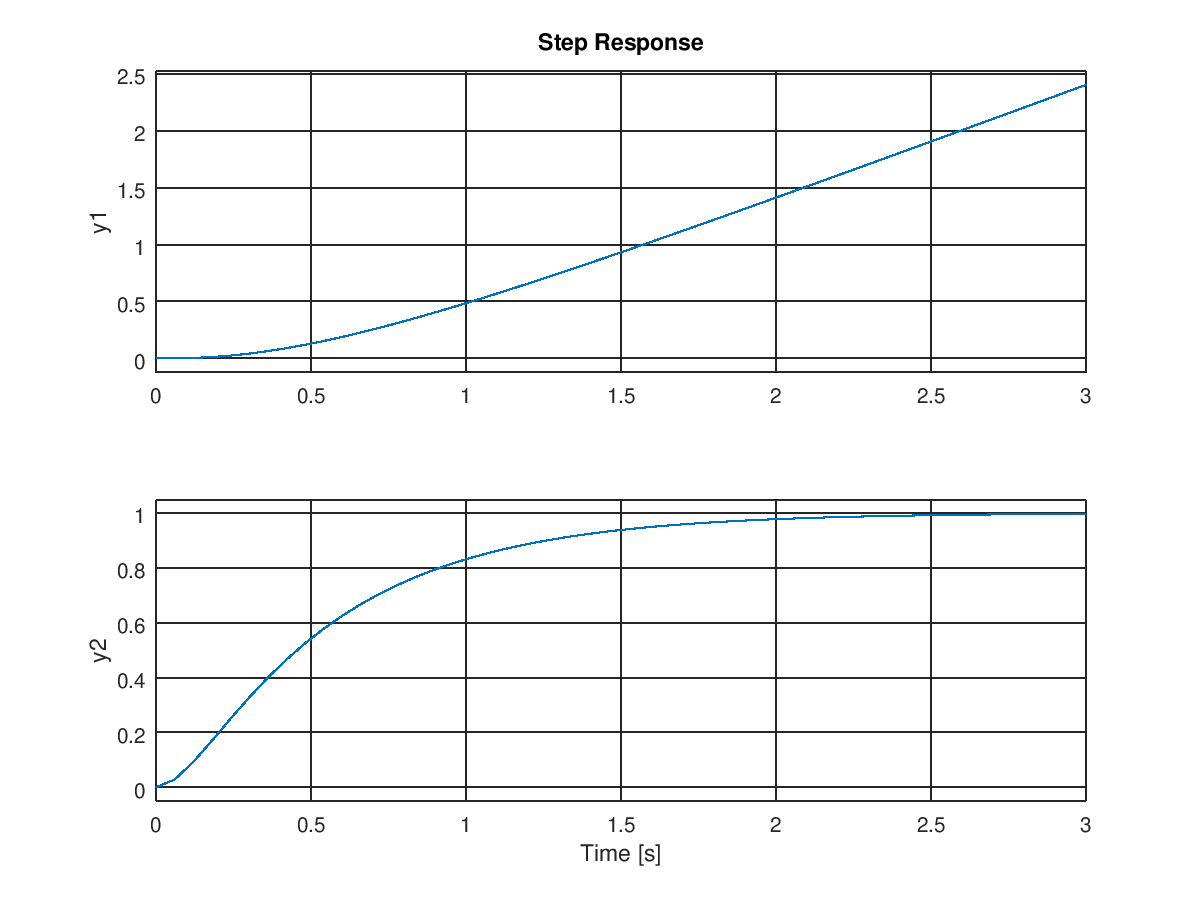
\includegraphics[width=\textwidth]{Images/question_2_output_response.png}
	\caption{Output response to a step input}
	\label{fig:question_2_output_response}
\end{figure}

Figure \ref{fig:question_2_output_response} shows the reponse of the sytem where $y_1$ is the angular displacement of the motor and $y_2$ is the angular speed of the motor. $y_1$ follows a linear relationship with time after transients of $y_2$ die out. This is expected seeing as though $y_2$ illustrates the rate of change of $y_1$, a constant rate of change (after roughly $2.5$ seconds) gives a linear relationship of the displacement. 

Before the transients die out, the displacement output $y_1$ shows to have a parabolic relationship with time. This is expected as the rate of change of disaplacement increases between the time $t=0$ seconds and $t=2.5$ seconds.    


\section{Question 3}

As given in the practical, the equation for current is slightly modified by
letting $\omega_r$ be evaluated as an error instead, due to the negative
feedback loop, thus replacing $\omega_r$ with $K_p[\omega_r(t) - \omega(t)]$.
The current equation then simply becomes

\begin{equation}
	\dot i = -\left[ \frac{K}{L} + \frac{K_P(Rb + K^2)}{LK} \right]\omega - \frac{R}{l}i + \frac{K_P(Rb + K^2)}{LK}\omega_r
	\label{eq:3_current}
\end{equation}

We can modify equation \eqref{eq:ss_position_eq1} to be

\begin{equation}
  \left[
  \begin{array}{c}
    \dot \theta \\
    \dot \omega \\
    \dot i
  \end{array}
  \right]
  =
  \left[
  \begin{array}{ccc}
    0 & 1 & 0 \\
    0 & -\frac{b}{J} & \frac{K}{J} \\
    0 & -\left[ \frac{K}{L} + \frac{K_P(Rb + K^2)}{LK} \right] & -\frac{R}{L}
  \end{array}
  \right]
  \left[
  \begin{array}{c}
    \theta \\
    \omega \\
    i
  \end{array}
  \right]
  +
  \left[
  \begin{array}{c}
    0 \\
    0 \\
    \frac{K_P(Rb + K^2)}{LK}
  \end{array}
  \right]
  \left[
  \begin{array}{c}
    \omega_r
  \end{array}
  \right]
  \label{eq:3_ss_position}
\end{equation}

The output system is exactly the same as in equation \eqref{eq:ss_position_eq2}.

\noindent
\texttt{J = 0.01;}\\
\texttt{b = 0.1;}\\
\texttt{K = 0.01;}\\
\texttt{R = 1;}\\
\texttt{L = 0.5;}\\
\texttt{A = [0,1,0;0,(-b/J),(K/J); 0 -((K/L)+(Kp\*(R\*b+K\^2)/L\*K)),-(R/L)];}\\
\texttt{B = [0;0;Kp\*(R\*b + K\^2)/(L\*K)];}\\
\texttt{C = [1,0,0;0,1,0];}\\
\texttt{D = [0;0];}\\
\texttt{[num,den] = ss2tf(A,B,C,D)}\\
\texttt{speed = tf(num(2),den(2));}\\
\texttt{step(feedback(speed));}\\
\texttt{s = tf('s');}\\
\texttt{position = feedback(speed) \* 1/s;}\\
\texttt{figure;}\\
\texttt{step(position);}\\

Shown below are the responses of the speed and the position of the DC motor respectively

\begin{figure}[H]
	\centering
	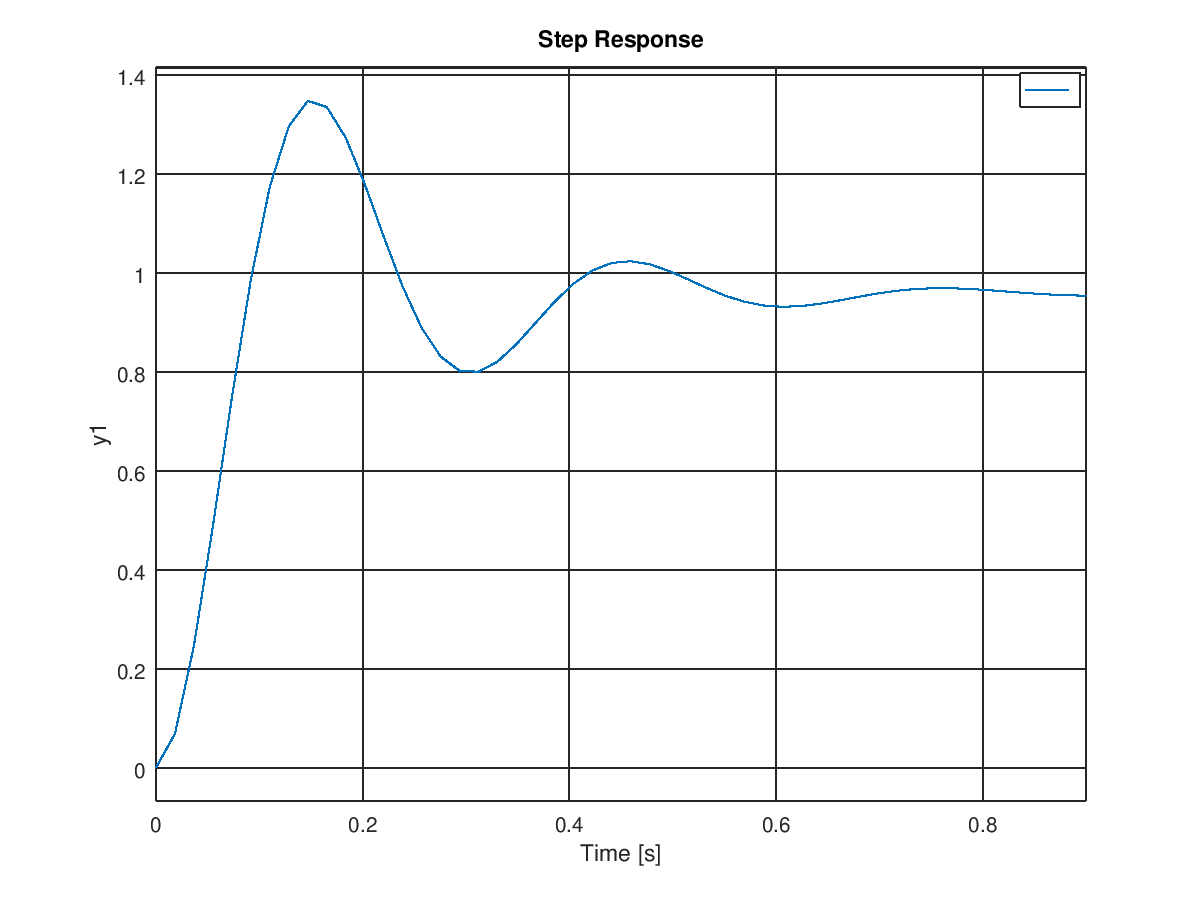
\includegraphics[width=\textwidth]{Images/question_3_speed.png}
	\caption{Output response of the speed of the DC motor}
	\label{fig:question_3_speed}
\end{figure}

\begin{figure}[H]
	\centering
	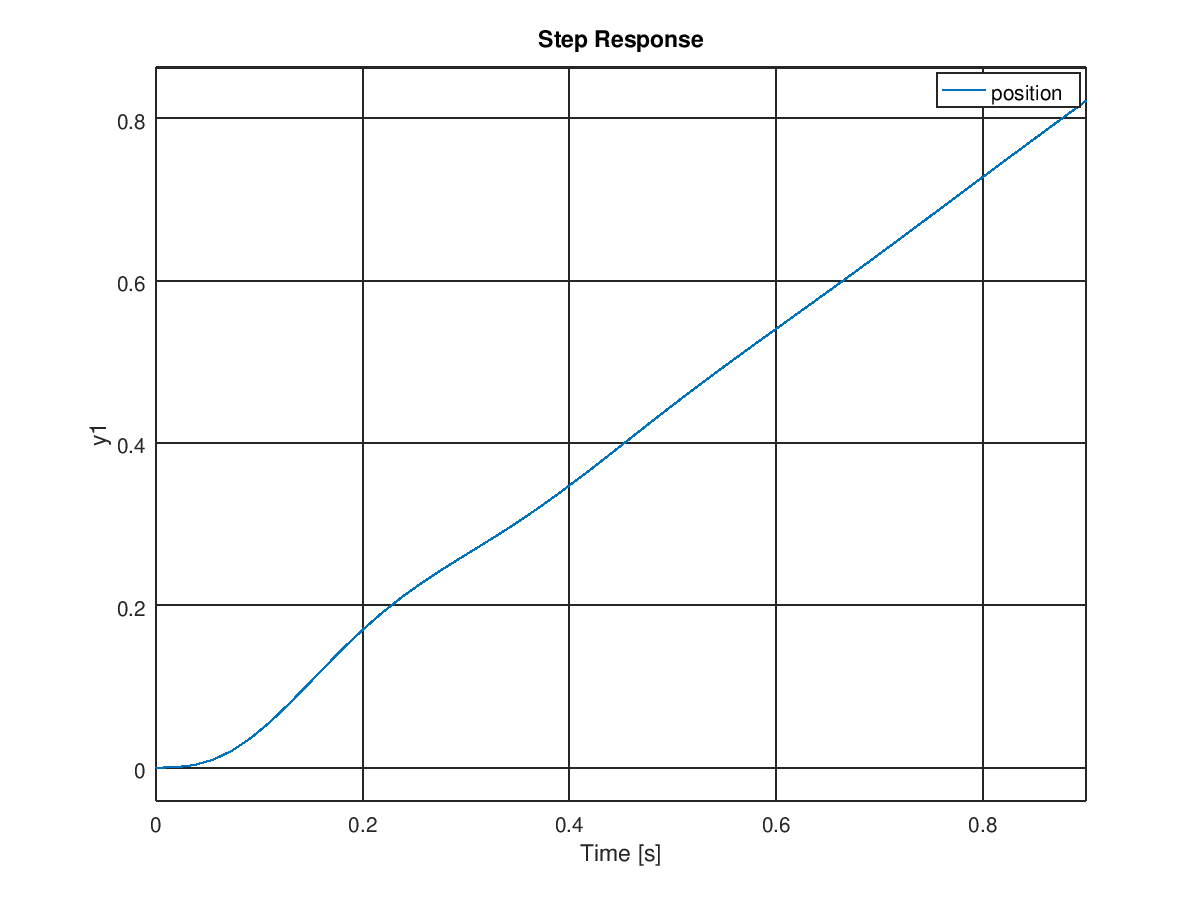
\includegraphics[width=\textwidth]{Images/question_3_pos.png}
	\caption{Output response of the position of the DC motor}
	\label{fig:question_3_pos}
\end{figure}

From these figures we deduce that the speed was achieved in a faster time frame (i.e. $t_s$ increased) which is the expected result of the addition of a proportional controller. The position plot of the motor (shown by Figure \ref{fig:question_3_pos}) has a linear relationship with time only after roughly $0.2$ seconds. This happens after this time due to the transients from the speed of the motor (Figure \ref{fig:question_3_speed}) that die out after $0.2$ seconds. 

\section{Question 4} % (fold)
\label{sec:question_4}

The derivation for the transfer function of this DC Motor has been derived in a
previous section, and given by equation \eqref{eq:ts_final}, which relates
input reference speed to the output speed of the motor. However, this is a
simple transfer function, and doesn't incorporate our control system. From
theory, the proper way to implement a control system with a contoller is to
feed it the error between the reference (commanding) signal and the actual
value being controlled from the system; in our case, $\omega_r - \omega$, and
then send this control signal into the $T(s)$, which will be equal to equation
\eqref{eq:ts_final}. Finally, the error is obtained with means of a negative
feedback loop. Thus, our output system in block diagram would look like this:

% lekker fokken diagram hier

with $E(s), U(s), D(s)$ being the laplace transform of our error signal,
control signal, and controller respectively, $\Omega_r(s)$ is the Laplace
transform of the reference speed, and $\Omega(s)$ is the Laplace transform of
the actual output speed of the motor.
\\

The code that produces the proportional and integral controller applied to the
system with transfer function $\frac{Rb+K^2}{(JL)s^3+(Lb+RJ)s+Rb+K}$ is shown
below \\ 
\noindent
\texttt{J = 0.012;}\\
\texttt{b = 0.105;}\\
\texttt{K = 0.01;}\\
\texttt{R = 1;}\\
\texttt{L = 0.505;}\\
\texttt{G = tf([R\*b+K\^2],[J\*L (L\*b+R\*J) R\*b+K]);}\\
\texttt{D = tf([Kd Kp Ki],[1 0])}\\
\texttt{H = feedback(D \* G)}\\
\texttt{step(H)}\\

Now applying the PI, PD and the PID controllers to the system with the desired design parameters.

\subsection{PI Controller} % (fold)
\label{sub:pi_controller}
By feeding the function (containing the code discussed in the beginning of this section) the values $K_p = 5, K_I = 8$ and $K_d = 0$ gave the response shown in Figure \ref{fig:question_4_pi}

\begin{figure}[H]
	\centering
	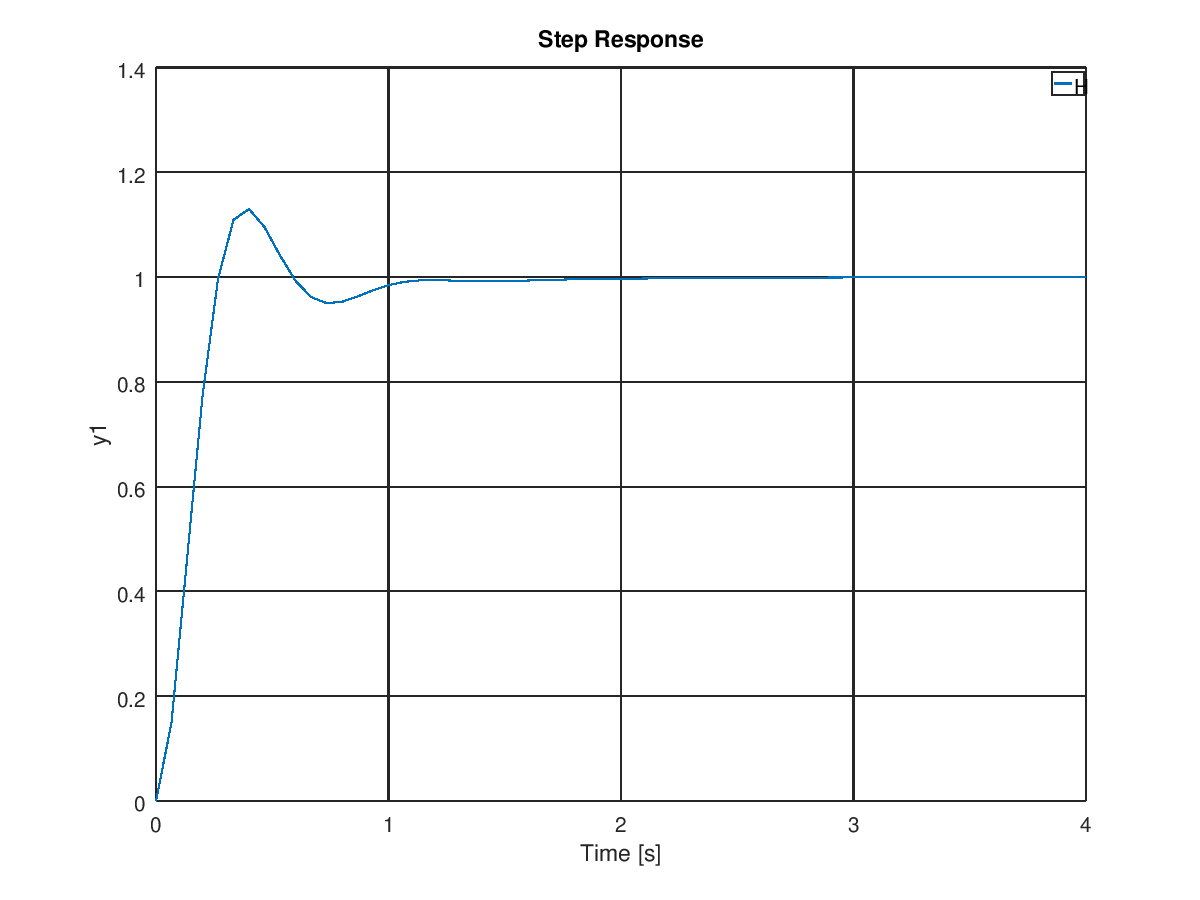
\includegraphics[width=\textwidth]{Images/question_4_PI.png}
	\caption{PI implementation with $K_p = 5, K_I = 8$ and $K_d = 0$}
	\label{fig:question_4_pi}
\end{figure}

This system gave us the specifications as defined below within spec of the design to be met
\begin{enumerate}
	\item $OS = 13\%$
	\item $t_s = 0.733$
	\item $\varepsilon = 0$
\end{enumerate}

% subsection pi_controller (end)

\subsection{PD Controller} % (fold)
\label{sub:pd_controller}
By feeding the function (containing the code discussed in the beginning of this section) the values $K_p = 29, K_I = 0$ and $K_d = 5$ gave the response shown in Figure \ref{fig:question_4_pd}

\begin{figure}[H]
	\centering
	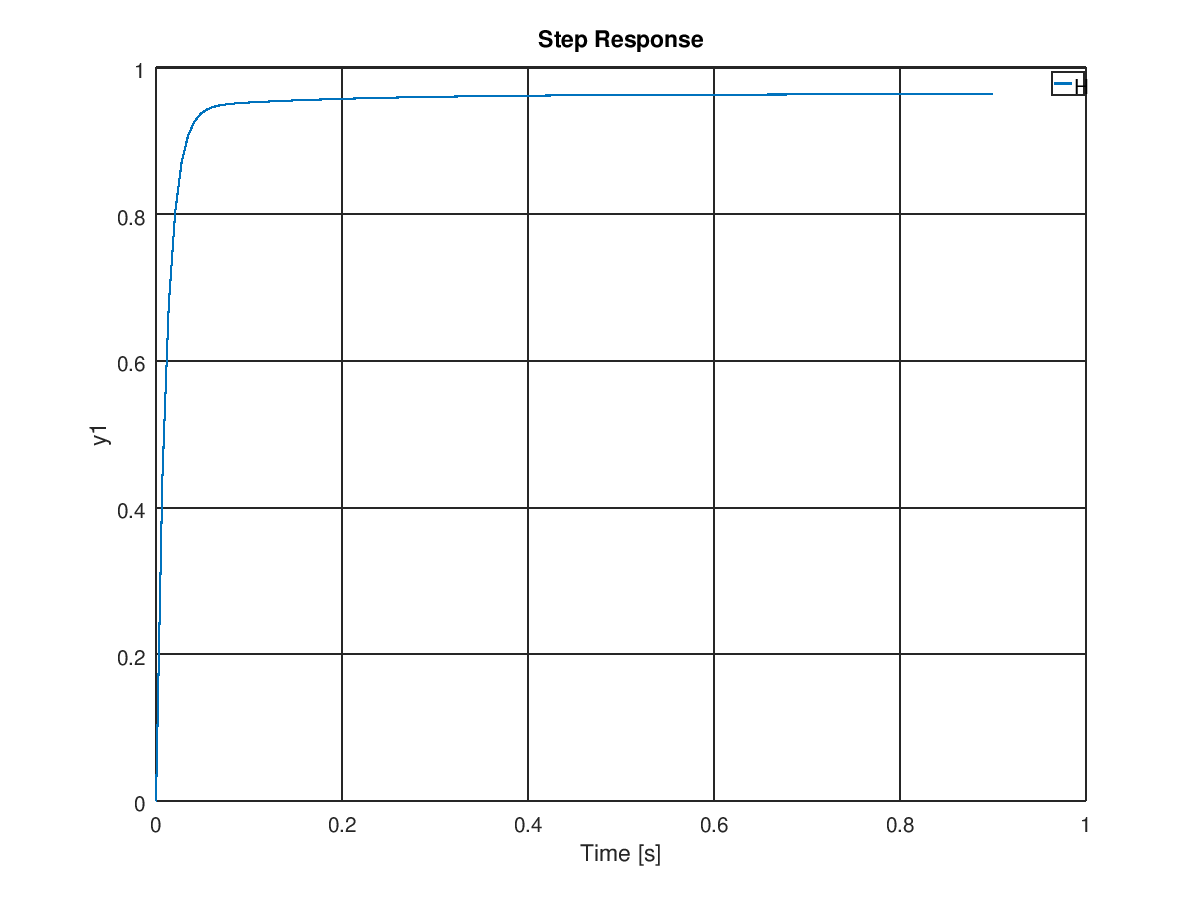
\includegraphics[width=\textwidth]{Images/question_4_PD.png}
	\caption{PD implementation with $K_p = 29, K_I = 0$ and $K_d = 5$}
	\label{fig:question_4_pd}
\end{figure}

This system gave us the specifications as defined below within spec of the design to be met
\begin{enumerate}
	\item $OS = 0\%$
	\item $t_s = 0.07$
	\item $\varepsilon = 4\%$
\end{enumerate}

% subsection pd_controller (end)

\subsection{PID Controller} % (fold)
\label{sub:pid_controller}
By feeding the function (containing the code discussed in the beginning of this section) the values $K_p = 5, K_I = 10$ and $K_d = 0.8$ gave the response shown in Figure \ref{fig:question_4_pid}

\begin{figure}[H]
	\centering
	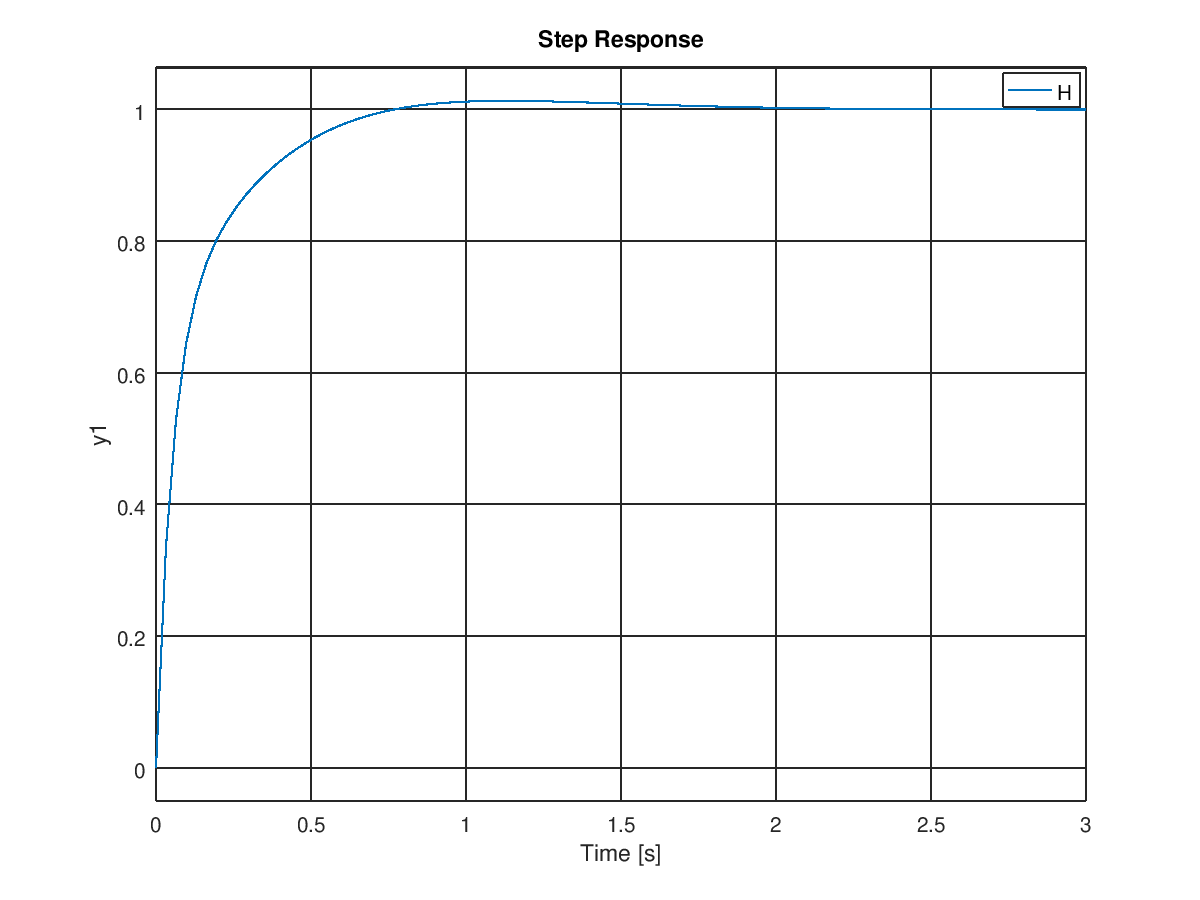
\includegraphics[width=\textwidth]{Images/question_4_PID.png}
	\caption{PID implementation with $K_p = 5, K_I = 10$ and $K_d = 0.8$}
	\label{fig:question_4_pid}
\end{figure}

This system gave us the specifications as defined below within spec of the design to be met
\begin{enumerate}
	\item $OS = 2\%$
	\item $t_s = 0.489$
	\item $\varepsilon = 0$
\end{enumerate}
% subsection id_controller (end)


% section question_4 (end)


\end{document}

